\chapter{El LHC y el experimento ATLAS}
\label{ch:atlas}
\epigraph{\emph{``Any sufficiently advanced technology is indistinguishable from magic."}}{Arthur C. Clarke}



El trabajo de esta tesis se ha realizado utilizando datos del detector \ac{ATLAS}, uno de los detectores de partículas que registran colisiones de protones acelerados por el \acf{LHC} en la \ac{CERN}.
En el presente capítulo, se ofrece una introducción al \ac{LHC} en la \Sect{\ref{sec:atlas:LHC}}, seguida de una discusión del detector \ac{ATLAS} en la \Sect{\ref{sec:atlas:atlas}}. Finalmente, en la \Sect{\ref{sec:atlas:runs}}, se describe brevemente cuáles fueron las condiciones para la toma de datos de \ac{ATLAS}, así como también sus propiedades. La discusión se centra en aspectos importantes para los análisis de esta tesis.




\section{LHC}
\label{sec:atlas:LHC}

El \ac{LHC} \cite{LHC-TDR,LHC-Machine} es el mayor acelerador de hadrones del mundo, situado en el \ac{CERN}, en la frontera franco-suiza. Tiene una longitud de 27 km y está situado entre 50 y 174 metros bajo tierra.
El \ac{LHC} está diseñado para hacer colisionar protones a una energía de centro de masa de \(14~\tev\). Para mantener los protones y los iones pesados en el anillo del acelerador, se utilizan un total de 9593 imanes. Este sistema incluye imanes superconductores dipolares y cuadrupolares, enfriados a 1.9 K (-271 $^{\circ} C$), de los cuales los imanes dipolares generan un campo magnético de 8.3 T.

\begin{figure}[ht!]
    \centering
    \includegraphics[width=0.75\linewidth]{3_experiment/lhc/AcceleratorComplex2022_large.png}
    \caption{Vista general del complejo de aceleradores del \ac{LHC}~\cite{LHC-complex}.}
    \label{fig:atlas:lhc:lhc}
\end{figure}

En la \Fig{\ref{fig:atlas:lhc:lhc}} se muestra un esquema general de las instalaciones del acelerador \ac{LHC}. Los protones se obtienen de hidrógeno gaseoso eliminando sus electrones y se aceleran en un primer acelerador lineal (LINAC2) hasta \(50~\mev\). Posteriormente, los protones se aceleran sucesivamente en el \ac{PSB}, el \ac{PSync} y el \ac{SPS}, donde alcanzan una energía de \(450~\gev\) antes de ser inyectados en el \ac{LHC}. En el \ac{LHC}, 8 cavidades de radiofrecuencia pueden impulsar la energía de los protones hasta \(14~\tev\). Los cuatro puntos amarillos en la imagen \Fig{\ref{fig:atlas:lhc:lhc}} son cuatro puntos de interacción entre las partículas acelaradas, que albergan los experimentos \acused{ALICE}\acs{ALICE}~\cite{ALICE}, \acs{LHCb}\acused{LHCb}~\cite{LHCb}, \acs{CMS}\acused{CMS}~\cite{CMS}, \acs{ATLAS}\acused{ATLAS}~\cite{ATLAS}, \acs{LHCf}\acused{LHCf}~\cite{LHCf}, \acs{TOTEM}\acused{TOTEM}~\cite{TOTEM}, \acsu{MoEDAL}\acused{MoEDAL}~\cite{MoEDAL}, entre muchos otros.

Los protones se inyectan en paquetes (\textit{bunches}) de \(\mathcal{O}(10^{11})\) protones en el \ac{LHC} con una separación de 25 ns (7.5 m). Estos haces se llevan posteriormente a colisión en los llamados \textit{bunch-crossing}. El esquema de llenado de la cadena del preacelerador, en combinación con los tiempos de conmutación finitos de los imanes de inyección y descarga, da lugar a patrones regulares de paquetes llenos y vacíos.

% Hasta ahora, el \ac{LHC} ha proporcionado haces de protones e iones pesados durante dos periodos de toma de datos, y se está sometiendo a un tercero. Entre 2009 y 2013 (conocido como \RunOne), el \ac{LHC} operó con una energía de centro de masa ($\sqrt{s}$) de 7 TeV y 8 TeV. Tras la primera larga parada de toma de datos (\ac{LS1}), la segunda corrida (\RunTwo) comenzó en 2015 y finalizó en 2018, proporcionando colisiones de 13 TeV a los experimentos alrededor del anillo \ac{LHC}. En 2022 comenzó el Run-3, en el que se producen \pp colisiones a una energía de \(13.6~\tev\), que se estima durará hasta 2026.



Uno de los parámetros más importantes para caracterizar el funcionamiento del acelerador es la luminosidad instantánea \(\mathcal{L}\), definida como el número de partículas por unidad de tiempo por unidad de área, y puede calcularse a partir de la relación
\begin{equation}
    \mathcal{L} = \frac{N_b^ 2n_b f_{rev}\gamma_r}{4\pi\epsilon_n\beta^*}F
    \label{eq:atlas:LHC:instantaneous_lumi}
\end{equation}
donde $N_b$ es el número de partículas por bunch, $n_b$ el número de bunches por haz, $\gamma_r$ es el factor gamma relativista, $\epsilon_n$ es la emitancia transversal normalizada del haz y $\beta^*$ es la función beta en el punto de colisión que determina la dispersión transversal del haz de partículas. El término de corrección F tiene en cuenta el ángulo de cruce del haz. La frecuencia de revolución está representada por $f_{rev}$ que es de \(\sim 11~\)kHz, y con el espaciado del haz de \(25~ns\), permite el cruce del haz en los cuatro puntos de interacción con una frecuencia de \(\sim 40~\)MHz.

La medida para el total de datos registrados se obtiene a partir de la luminosidad integrada a lo largo del tiempo y viene dada por
\begin{equation}
    N_{event} = L_{int} \sigma_{event} = \sigma_{event} \int \mathcal{L} dt.
    \label{eq:atlas:LHC:integrated_lumi}
\end{equation}
Esta variable relaciona la luminosidad con el número de eventos. Más detalles sobre las mediciones de luminosidad en \ac{ATLAS} se muestran en \Sect{\ref{sec:atlas:runs}}.








\FloatBarrier
\section{ATLAS}
\label{sec:atlas:atlas}

\ac{ATLAS} es uno de los detectores multipropósito del \ac{LHC}. Fue diseñado y construido para estudiar las colisiones \pp (y de iones pesados) y un gran espectro de procesos físicos en la escalade energía del \tev.

La forma general del detector es la de un cilindro, como se muestra en la \Fig{\ref{fig:atlas:atlas:atlas}}. Tiene una longitud de 44 m y 25 m de diámetro, siendo el mayor detector de partículas construido hasta la fecha. El detector \ac{ATLAS} está dividido geométricamente en dos partes: la parte central (\textit{barrel}), y las tapas exteriores (\textit{end-caps}).

\begin{figure}[ht!]
    \centering
    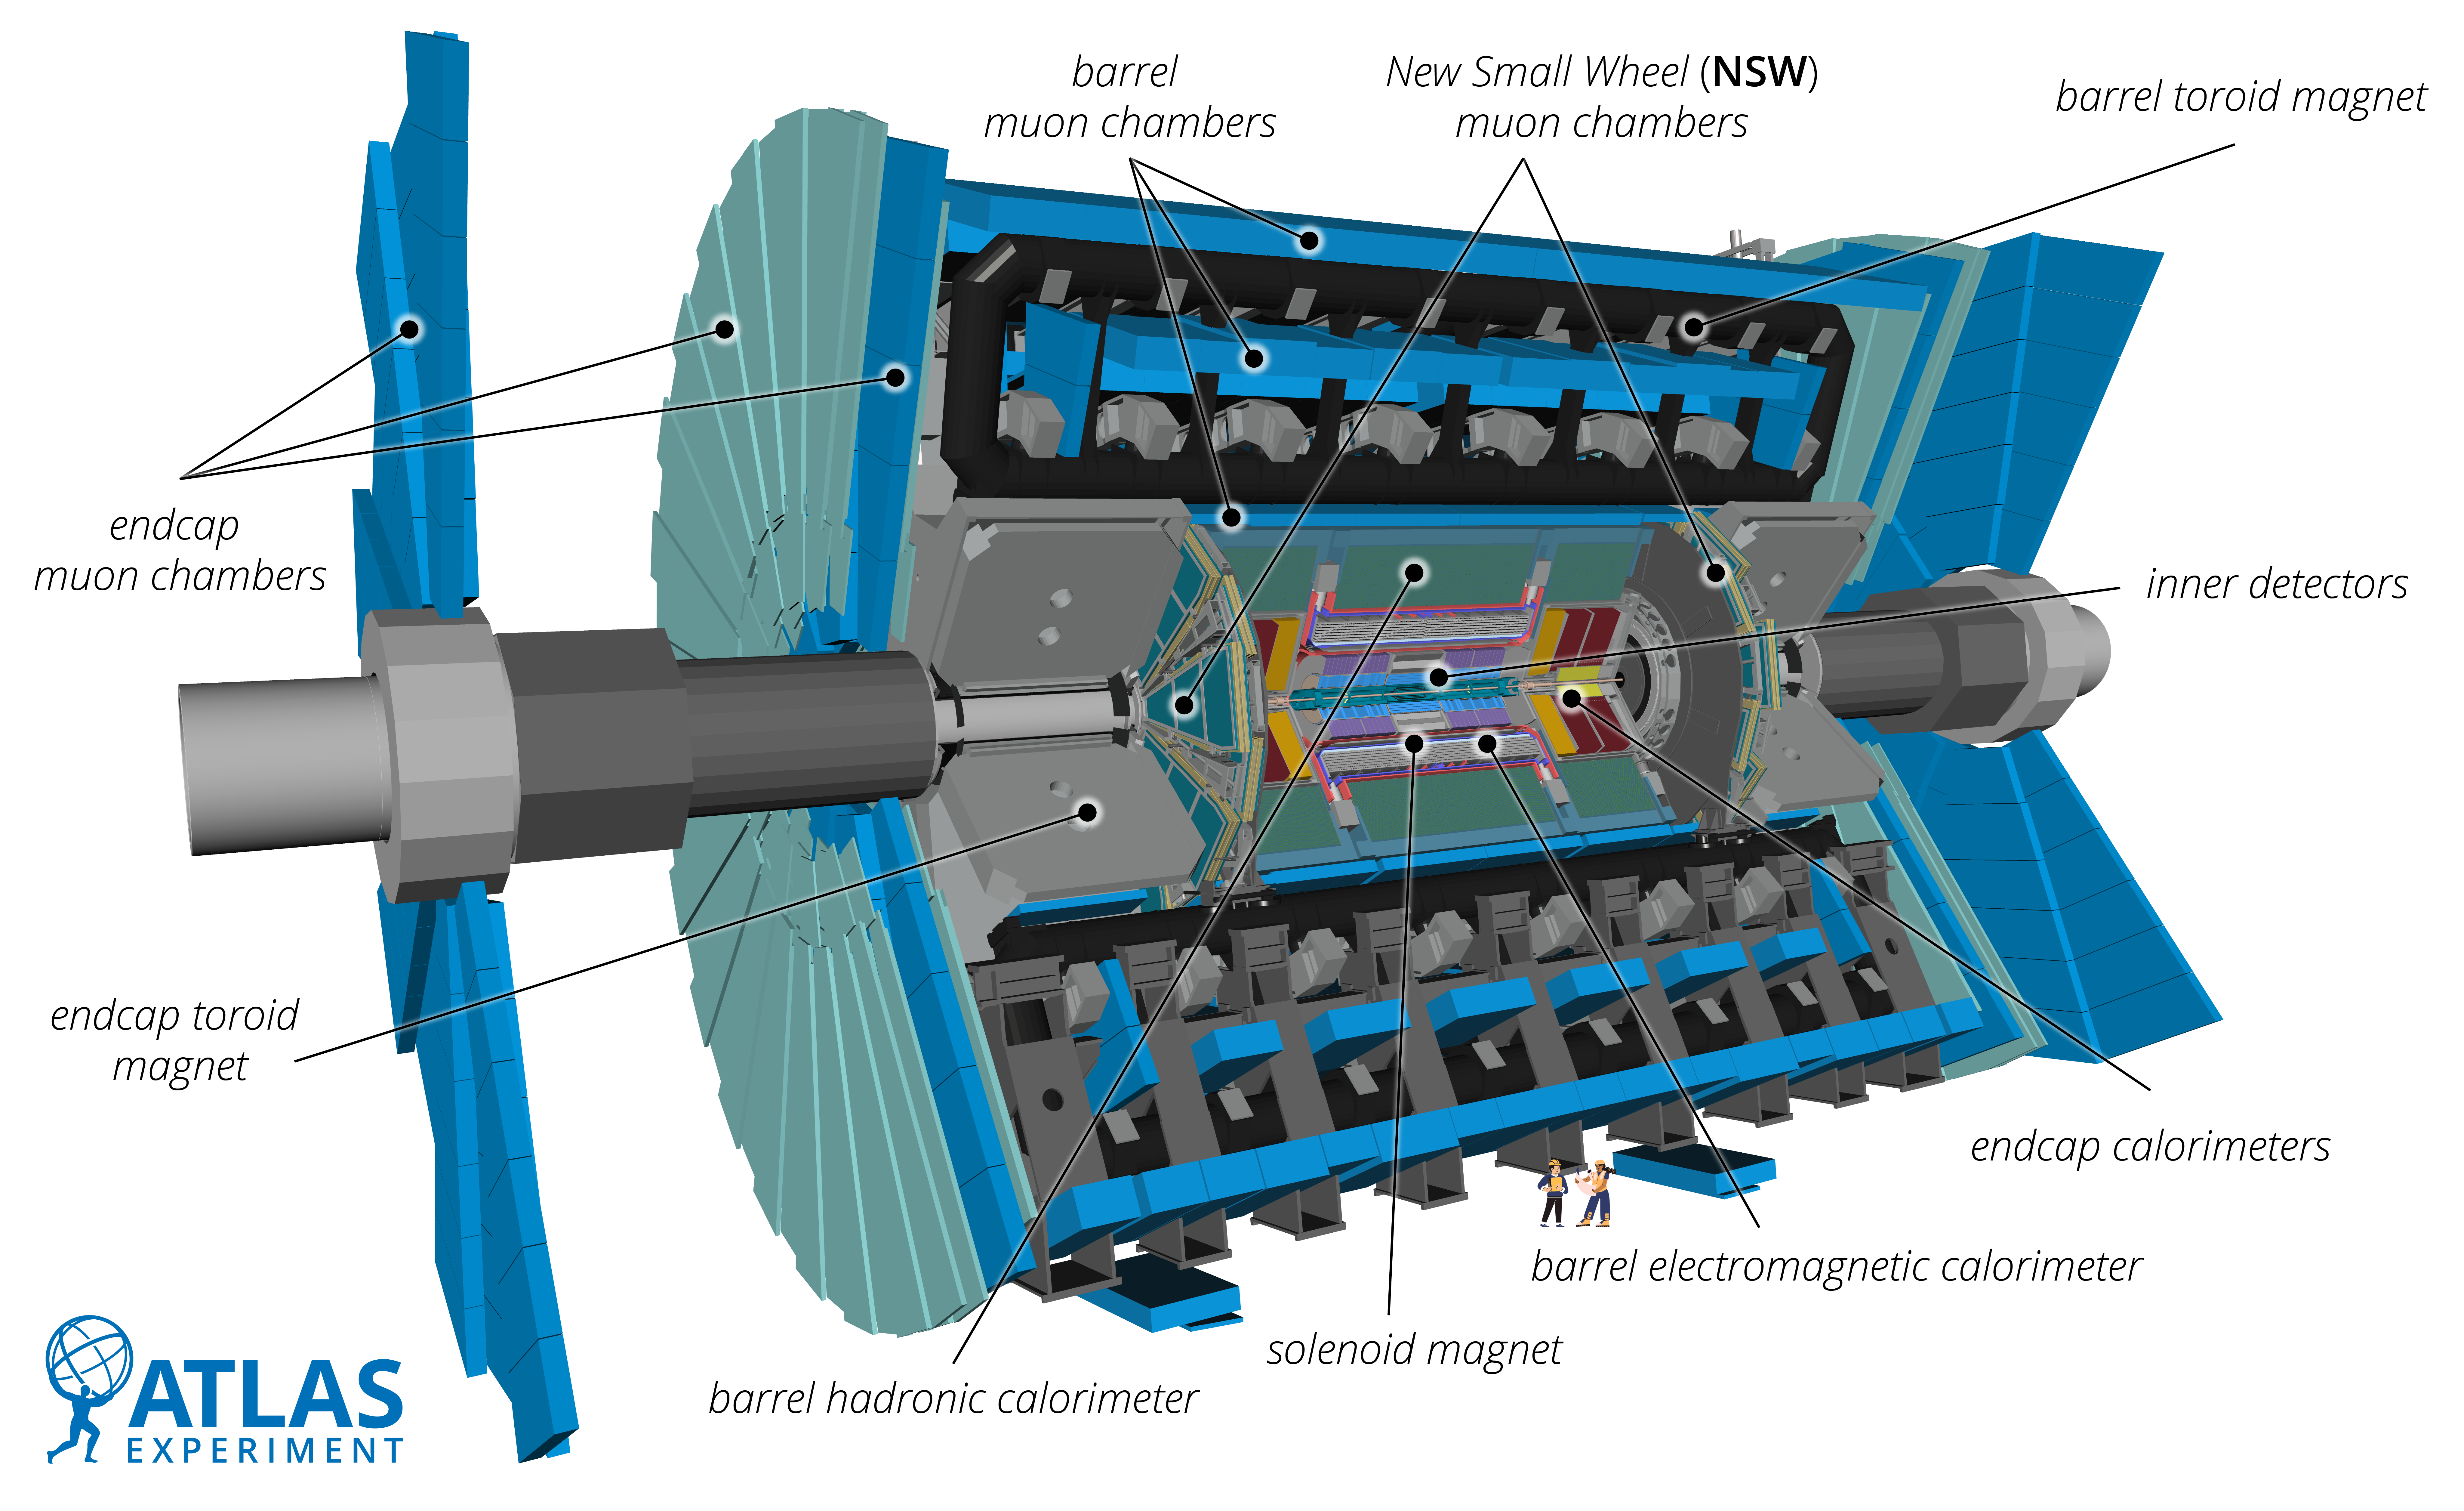
\includegraphics[width=0.8\linewidth]{3_experiment/atlas/ATLAS_full.png}
    \caption{Vista general del detector \ac{ATLAS} y de todos sus subdetectores, incluidos los sistemas añadidos durante el \ac{LS2}~\cite{ATLAS-Diagram}.}
    \label{fig:atlas:atlas:atlas}
\end{figure}

\ac{ATLAS} está construido en capas de subdetectores, cada uno de los cuales está diseñado para tener un papel diferente en la identificación y reconstrucción de las partículas producidas en las colisiones. \ac{ATLAS} proporciona una cobertura hermética alrededor del eje del haz, permitiendo la detección de todas las partículas cargadas generadas en las colisiones en el plano ortogonal al eje del haz. Esto es particularmente importante en las búsquedas de nueva física, que se basan en análisis de balances de momento en el plano ortogonal.

Está formado por múltiples capas, empezando por el componente más interno, el \acf{ID}, que permite reconstruir trazas cerca del tubo del haz. Alrededor del \ac{ID}, hay un solenoide superconductor que crea un campo magnético axial de \(\sim 2\) T para curvar las trazas de las partículas cargadas.
Tras este imán, hay un sistema de dos calorímetros: el \acf{ECAL} y el \acf{HCAL}. El primero se encarga de medir la energía cinética de fotones y electrones, y el segundo mide la energía de los jets.
Las partes más externas del \ac{ATLAS} están constituidas por el \acf{MS}, que proporciona la reconstrucción del momento de los muones que atraviesan las capas internas del detector. Entrelazadas con el \ac{MS}, hay un total de 8 bobinas toroidales que proporcionan un campo magnético total de 4 T para medir el momento de los muones. El campo magnético de los toroides se completa con los toroides en las regiones del end-cap, que también generan un campo magnético de hasta 4 T para los muones que salen en la dirección más próxima al haz.

% El trabajo conjunto de todos los componentes de \ac{ATLAS} permite reconstruir e identificar una gran variedad de partículas con gran precisión. En la \Tab{\ref{tab:atlas:atlas:expected_performance}}, adaptado de \Refn{\cite{ATLAS}}, se da una visión general de las capacidades de diseño de \ac{ATLAS} en términos de resolución de momento y energía.
% Aquí, la resolución está dada primero por un término estocástico, que mide la incertidumbre basada en la interacción de una partícula con el material, seguido de un término de ruido, que da cuenta de las incertidumbres debidas al ruido electrónico en el proceso de lectura.




% \begin{table}[ht!]
%     \caption{Rendimiento esperado del detector \ac{ATLAS}. Las unidades de \pt y \(E\) están en \gev. Extraído de \Refn{\cite{ATLAS}}}
%     \begin{tabular}{|l|c|c|c|}
%         \hline
%         \multirow{2}{*}{\textbf{Componente del detector}}    & \multirow{2}{*}{\textbf{Resolución requerida}}     & \multicolumn{2}{c|}{\textbf{Cobertura en $\eta$}}             \\\cline{3-4} 
%                                                         &                                                   & Offline               & Trigger                        \\ \hline
%         \ac{ID}                                        & \( \sigma_{\pt}/\pt = 0.05\%\pt \oplus 1\%    \)  & \( \pm 2.5 \)            &                                \\ \hline
%         \ac{ECAL}                                  & \( \sigma_{E}/E = 10\%/\sqrt{E} \oplus 0.7\%  \)  & \( \pm 3.2 \)            & \( \pm 2.5 \)                  \\ \hline
%         \ac{HCAL} (jets)                     &                                                   &                          &                                \\
%         $\quad$ barrel y end-cap                       & \( \sigma_{E}/E = 50\%/\sqrt{E} \oplus 3\%    \)  & \( \pm 3.2 \)            & \( \pm 3.2 \)                  \\
%         $\quad$ dirección forward                                  & \( \sigma_{E}/E = 100\%/\sqrt{E} \oplus 10\%  \)  & \( 3.1 < \abseta< 4.9 \) & \( 3.1 < \abseta< 4.9 \)       \\ \hline
%         \ac{MS}                               & \( \sigma_{\pt}/\pt = 10\%\) at \(\pt =1~\tev \)  & \( \pm 2.7 \)            & \( \pm 2.4 \)                  \\
%         \hline
%     \end{tabular}
%     \label{tab:atlas:atlas:expected_performance}
% \end{table}







\subsection{Sistema de coordenadas de ATLAS}

\begin{figure}[ht!]
    \centering
    \includegraphics[width=0.8\linewidth]{3_experiment/atlas/ATLAS_coordinates}
    \caption{Sistema de coordenadas de \ac{ATLAS}~\cite{ATLAS-Diagram}.}
    \label{fig:atlas:atlas:atlas_coordinates}
\end{figure}

El sistema de coordenadas utilizado en \ac{ATLAS}, que se muestra en \Fig{\ref{fig:atlas:atlas:atlas_coordinates}}, se utiliza en toda esta tesis y se describe brevemente a continuación~\cite{ATLAS}.
El origen del sistema de coordenadas está en el punto de interacción nominal, con el eje x positivo apuntando hacia el centro del \ac{LHC}. El plano x-y es perpendicular al eje del haz, definiendo el eje z. Hacia la superficie define el eje y positivo. Alrededor del eje del haz se define un ángulo azimutal $\phi$, y un ángulo polar $\theta$ es el ángulo desde el eje del haz. En lugar de $\theta$ se utiliza la rapidez $y$ que para objetos pesados tiene la forma:
\begin{equation}
    y = \frac{1}{2} \ln[(E+p_z)/(E-p_z)].
\end{equation}
Las diferencias en la rapidez son invariantes a \textit{boosts} a lo largo del eje del haz. Para objetos sin masa o relativistas ($m \ll \vb*{p}$) se utiliza en su lugar la pseudorapidez:
\begin{equation}
    \eta = -\ln(\tan(\theta/2)).
\end{equation}
Para cuantificar la distancia entre dos objetos, se define \DeltaR:
\begin{equation}
    \DeltaR = \sqrt{\Delta\phi^2 + \Delta\eta^2}
\end{equation}
El momento transverso y la energía se definen en el plano x-y, con el momento transverso dado como $\pt = \sqrt{p_x^2 +p_y^2}$.






\subsection{Detector Interno}
\label{subsec:atlas:atlas:id}

\begin{figure}[ht!]
    \centering
    \begin{subfigure}[t]{0.49\linewidth}
        \centering
        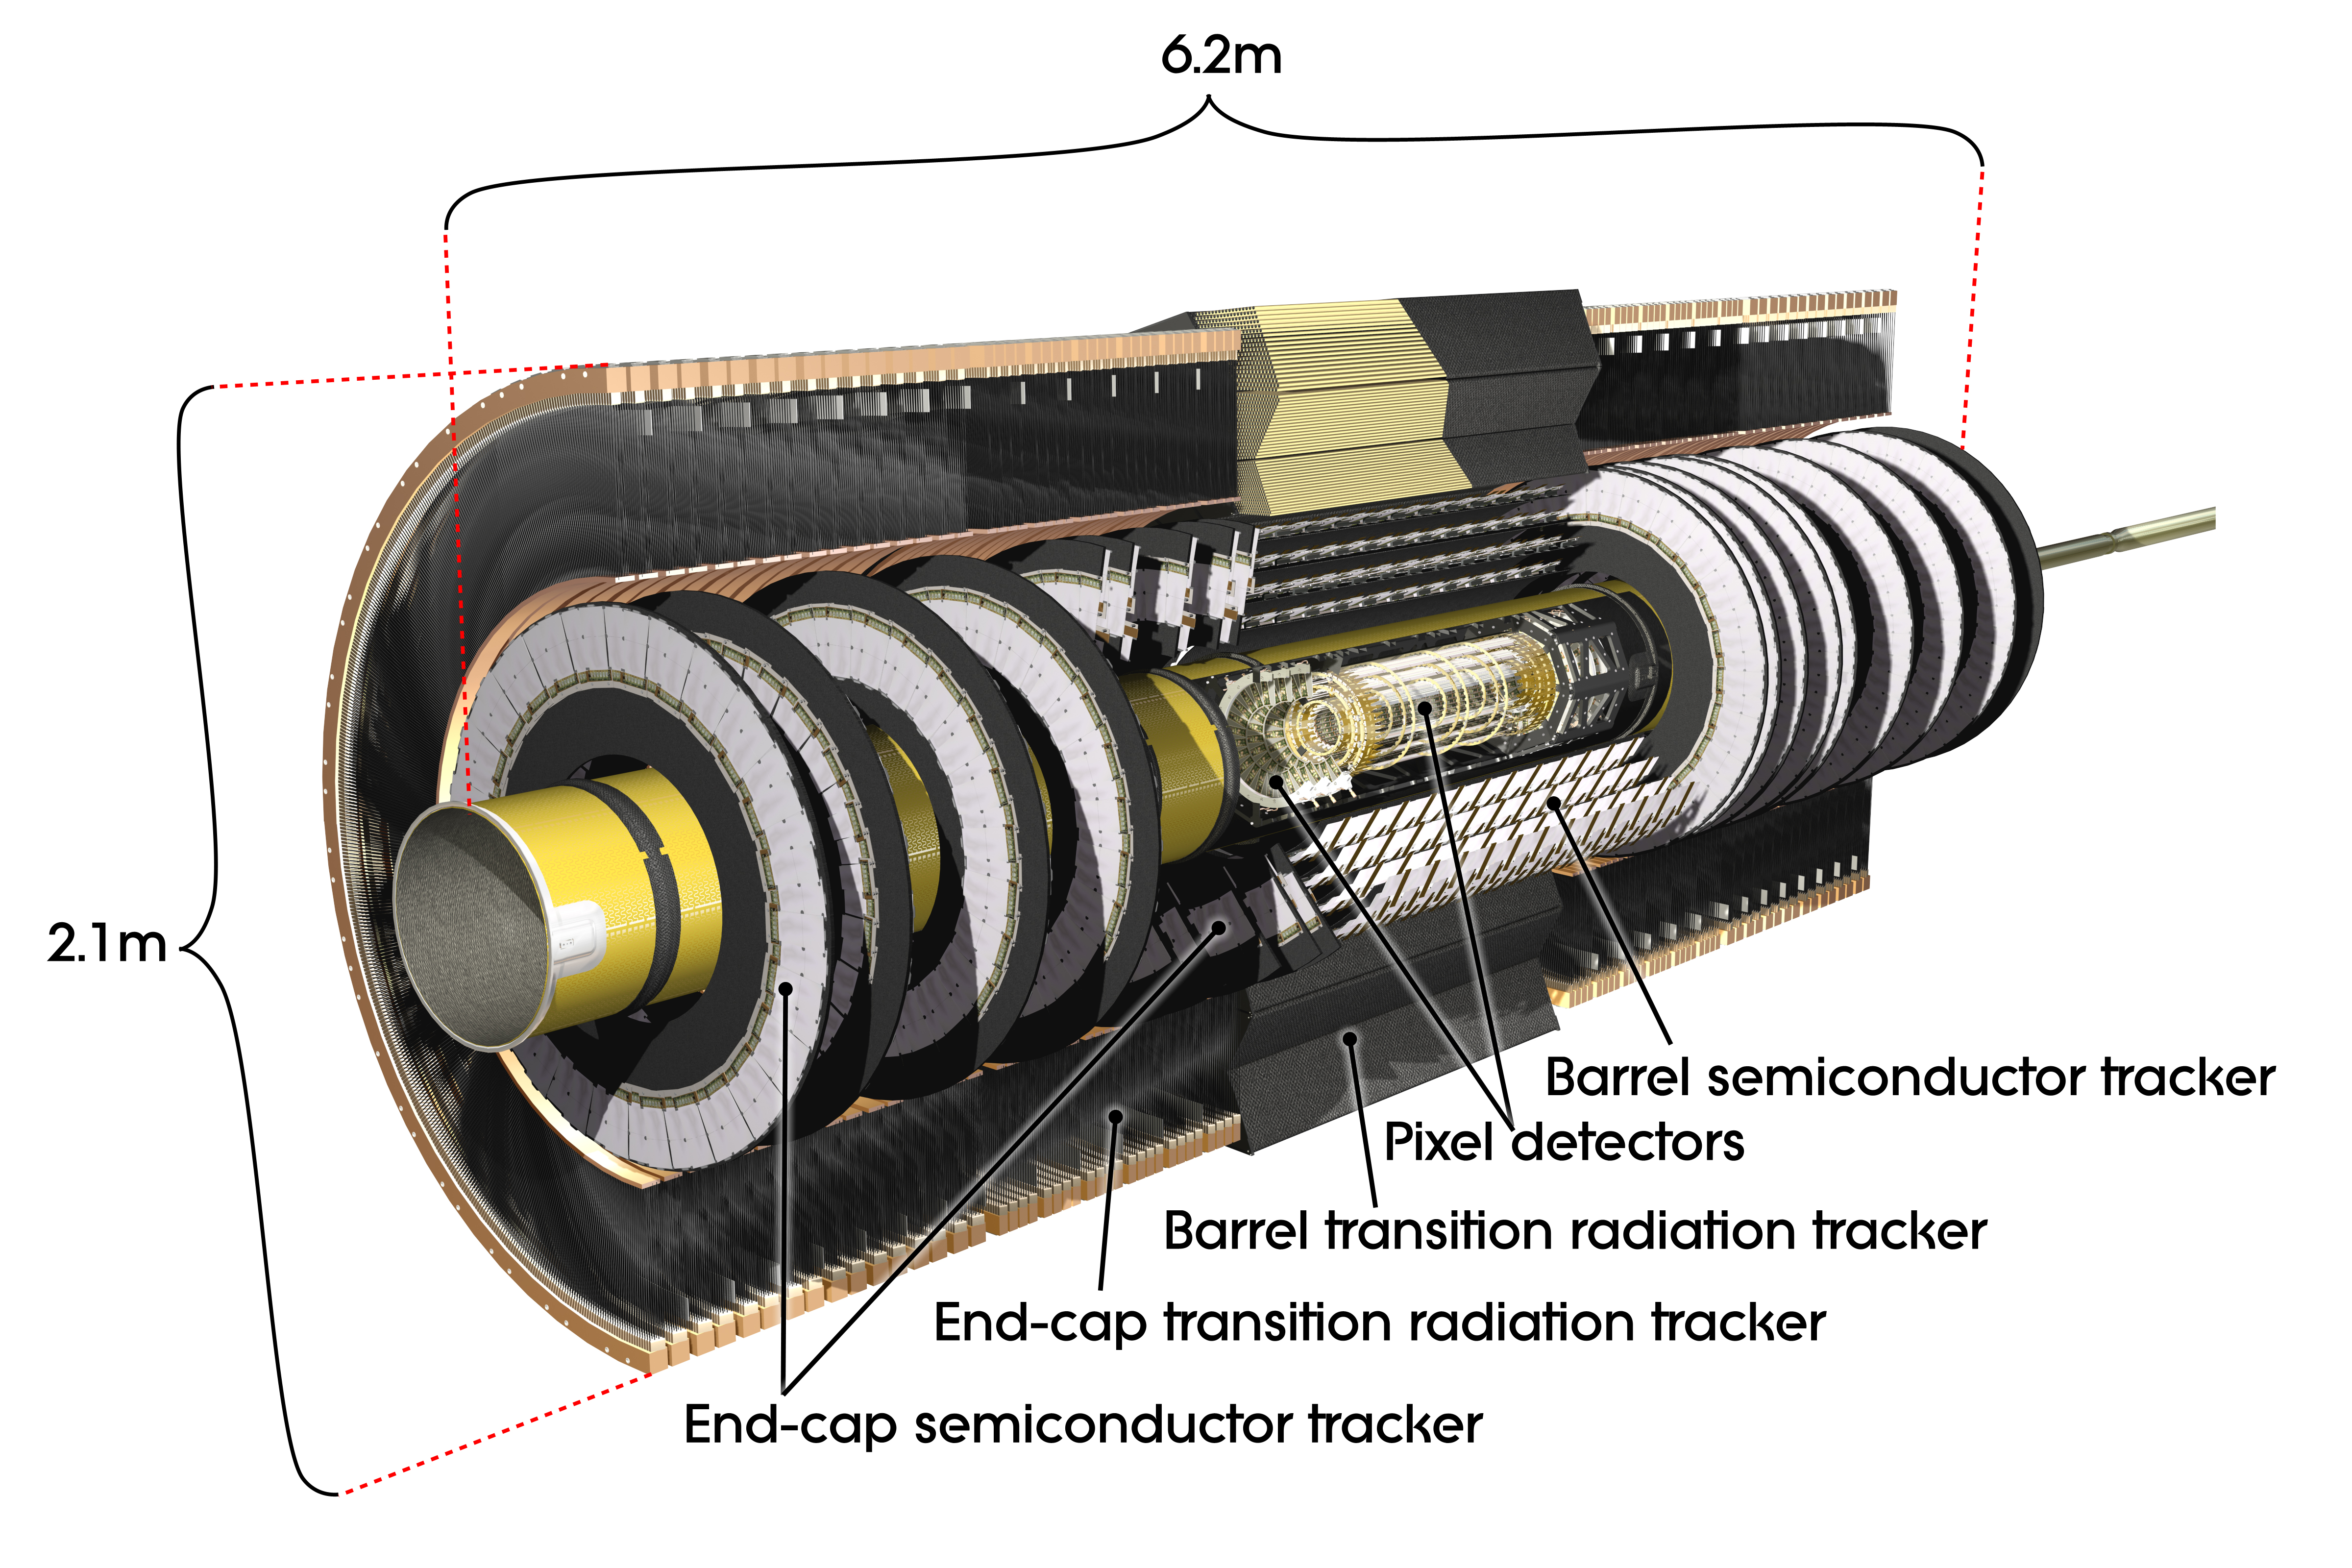
\includegraphics[width=\linewidth]{3_experiment/atlas/inner_detector.jpg}
        \caption{El \ac{ID} con todos sus submódulos en las regiones de barrel y end-cap.~\cite{ATLAS-InnerDetector}.}
        \label{fig:atlas:atlas:atlas_inner_detector:general}
    \end{subfigure}
    \hfill
    \begin{subfigure}[t]{0.49\linewidth}
        \centering
        \includegraphics[width=0.8\linewidth]{3_experiment/atlas/inner_detector_layers}
        \caption{Capas del \ac{ID} mostrando su distancia al haz~\cite{ATLAS-InnerDetector}.}
        \label{fig:atlas:atlas:atlas_inner_detector:layer_radius}
    \end{subfigure}
    \caption{Diagramas del \ac{ID} que muestran los diferentes submódulos, con sus correspondientes dimensiones.}
    \label{fig:atlas:atlas:atlas_inner_detector}
\end{figure}

El esquema de un corte transversal del \acf{ID} \cite{ATLAS-ID-TDR} se muestra en la \Fig{\ref{fig:atlas:atlas:atlas_inner_detector}}, resaltando la distancia de cada subsistema respecto al tubo del haz. La parte más interna del \ac{ID} se denomina \ac{IBL}, seguido de tres capas de detectores de píxeles. A 299 mm de distancia radial del tubo del haz, cuatro capas de módulos del \ac{SCT} se sitúan antes del \ac{TRT}, que amplía el tamaño total del \ac{ID} a un radio de 1082 mm. El \ac{ID} permite la reconstrucción de las trazas de partículas en un rango de $\abseta < 2.5$.


La función del \ac{ID} es la reconstrucción de las trazas de las partículas cargadas para determinar su carga y momento. Está inmerso en un campo magnético de 2 T generado por el sistema magnético del solenoide de \ac{ATLAS}, que curva las trayectorias de las partículas cargadas. El radio de curvatura es proporcional al momento de la partícula y su dirección distingue las cargas positivas de las negativas. Las trazas de las partículas detectadas permiten reconstruir los vértices de colisiones primarios, lo cual es importante para distinguir las colisiones de \textit{pile-up} (término que será descrito más adelante) de las colisiones de interés, y los vértices secundarios de decaimiento producidos por partículas de vida media larga, lo que es crucial para la identificación de, por ejemplo, mesones \(B\) o leptones \(\tau\). A continuación, se brinda una breve descripción de cada parte del \ac{ID}.


\paragraph{\acf{IBL}}
Después del Run-1, durante el \ac{LS1} en el período de 2013-2014, el sistema detector de píxeles fue sometido a mantenimiento y actualizaciones. Dentro de este conjunto de actualizaciones, una cuarta capa de píxeles a 3.3 cm de distancia del tubo del haz fue instalada~\cite{ATLAS-IBL-TDR,ATLAS-IBL-proceedings} y ha permitido mejoras significativas en la reconstrucción de vértices de interacción y la identificación de jets iniciados por quarks \(b\).


\paragraph{Detector de Píxeles}
La capa de píxeles más interna, el \ac{IBL}, está rodeada por tres capas de detectores de píxeles, dispuestas alrededor del tubo del haz~\cite{ATLAS-Pixel-DesignPerformance,ATLAS-Pixel-Performance-Proceedings}. El método de detección de partículas cargadas es la medición de cargas inducidas depositadas en una capa de silicio, producto de la ionización. La primera capa se encuentra a una distancia de 50.5 mm del centro del tubo del haz. Como se puede ver en la \Fig{\ref{fig:atlas:atlas:atlas_inner_detector:general}}, en la región del end-cap los detectores de píxeles consisten en 3 discos alrededor del tubo, aumentando la longitud del detector de píxeles del \ac{ID} a 1.4 m a lo largo del eje del haz. El detector de píxeles consta de un total de 1744 módulos de píxeles con un tamaño nominal de $50 ~\mu m \times 400 ~\mu m$ en el plano $(\phi, z)$, que comprenden más de 80 millones de canales de lectura.  
La parte de píxeles y \ac{IBL} del detector \ac{ATLAS} es crucial para la reconstrucción de trazas, ya que proporciona 4 puntos de medición (\textit{hits}) en todo el rango de cobertura de pseudorapidez ($|\eta| < 2.5.$).  

\paragraph{\acf{SCT}}
El detector de píxeles y \ac{IBL} se encuentran dentro de los módulos del \ac{SCT}~\cite{ATLAS-SCT}.  
Al igual que los módulos detectores de píxeles, los módulos del \ac{SCT} están basados en semiconductores, dispuestos en capas cilíndricas alrededor del tubo del haz en la región del barrel, formando discos en los end-caps. Dado que los módulos del \ac{SCT} sólo proporcionan una localización precisa a lo largo de un eje, se combinan dos módulos uno detrás de otro y rotados entre sí para obtener información espacial bidimensional. En el barrel hay cuatro capas y en los end-caps, nueve discos en cada lado (véase la \Fig{\ref{fig:atlas:atlas:atlas_inner_detector:general}}). Incluyendo los discos de los end-caps, el \ac{SCT} se extiende hasta $|z| < 2735~mm$.

\paragraph{\acf{TRT}}
La última parte del \ac{ID} es el \ac{TRT}~\cite{ATLAS-TRT-DesignPerformance}, el cual en la región barrel se extiende de 554 mm a 1082 mm de distancia radial. Este detector se compone de tubos detectores de 4 mm de diámetro, dispuestos en paralelo al tubo del haz en la región barrel, y radialmente en los end-caps. En el rango de $|\eta| < 2.0$, se sitúan tres anillos en el barrel y 18 unidades en los end-caps, proporcionando típicamente 36 impactos por traza. Los tubos están entrelazadas con fibras de polipropileno, que cuando las partículas las atraviesan, crean la radiación de transición. En el interior de los tubos hay un fino cable de tungsteno que recoge las cargas. El nivel de radiación y las cargas recogidas en cada tubo pueden utilizarse para discriminar entre electrones y piones cargados. El \ac{TRT} sólo ofrece información espacial en el plano $(R-\phi)$, y no se puede extraer información en la dirección z debido a la orientación de estos tubos. Hay un total de aproximadamente 50000 tubos en la región del barrel, mientras que en los end-caps se sitúan aproximadamente 250000 tubos.








\subsection{Calorímetros}

\begin{figure}[ht!]
    \centering
    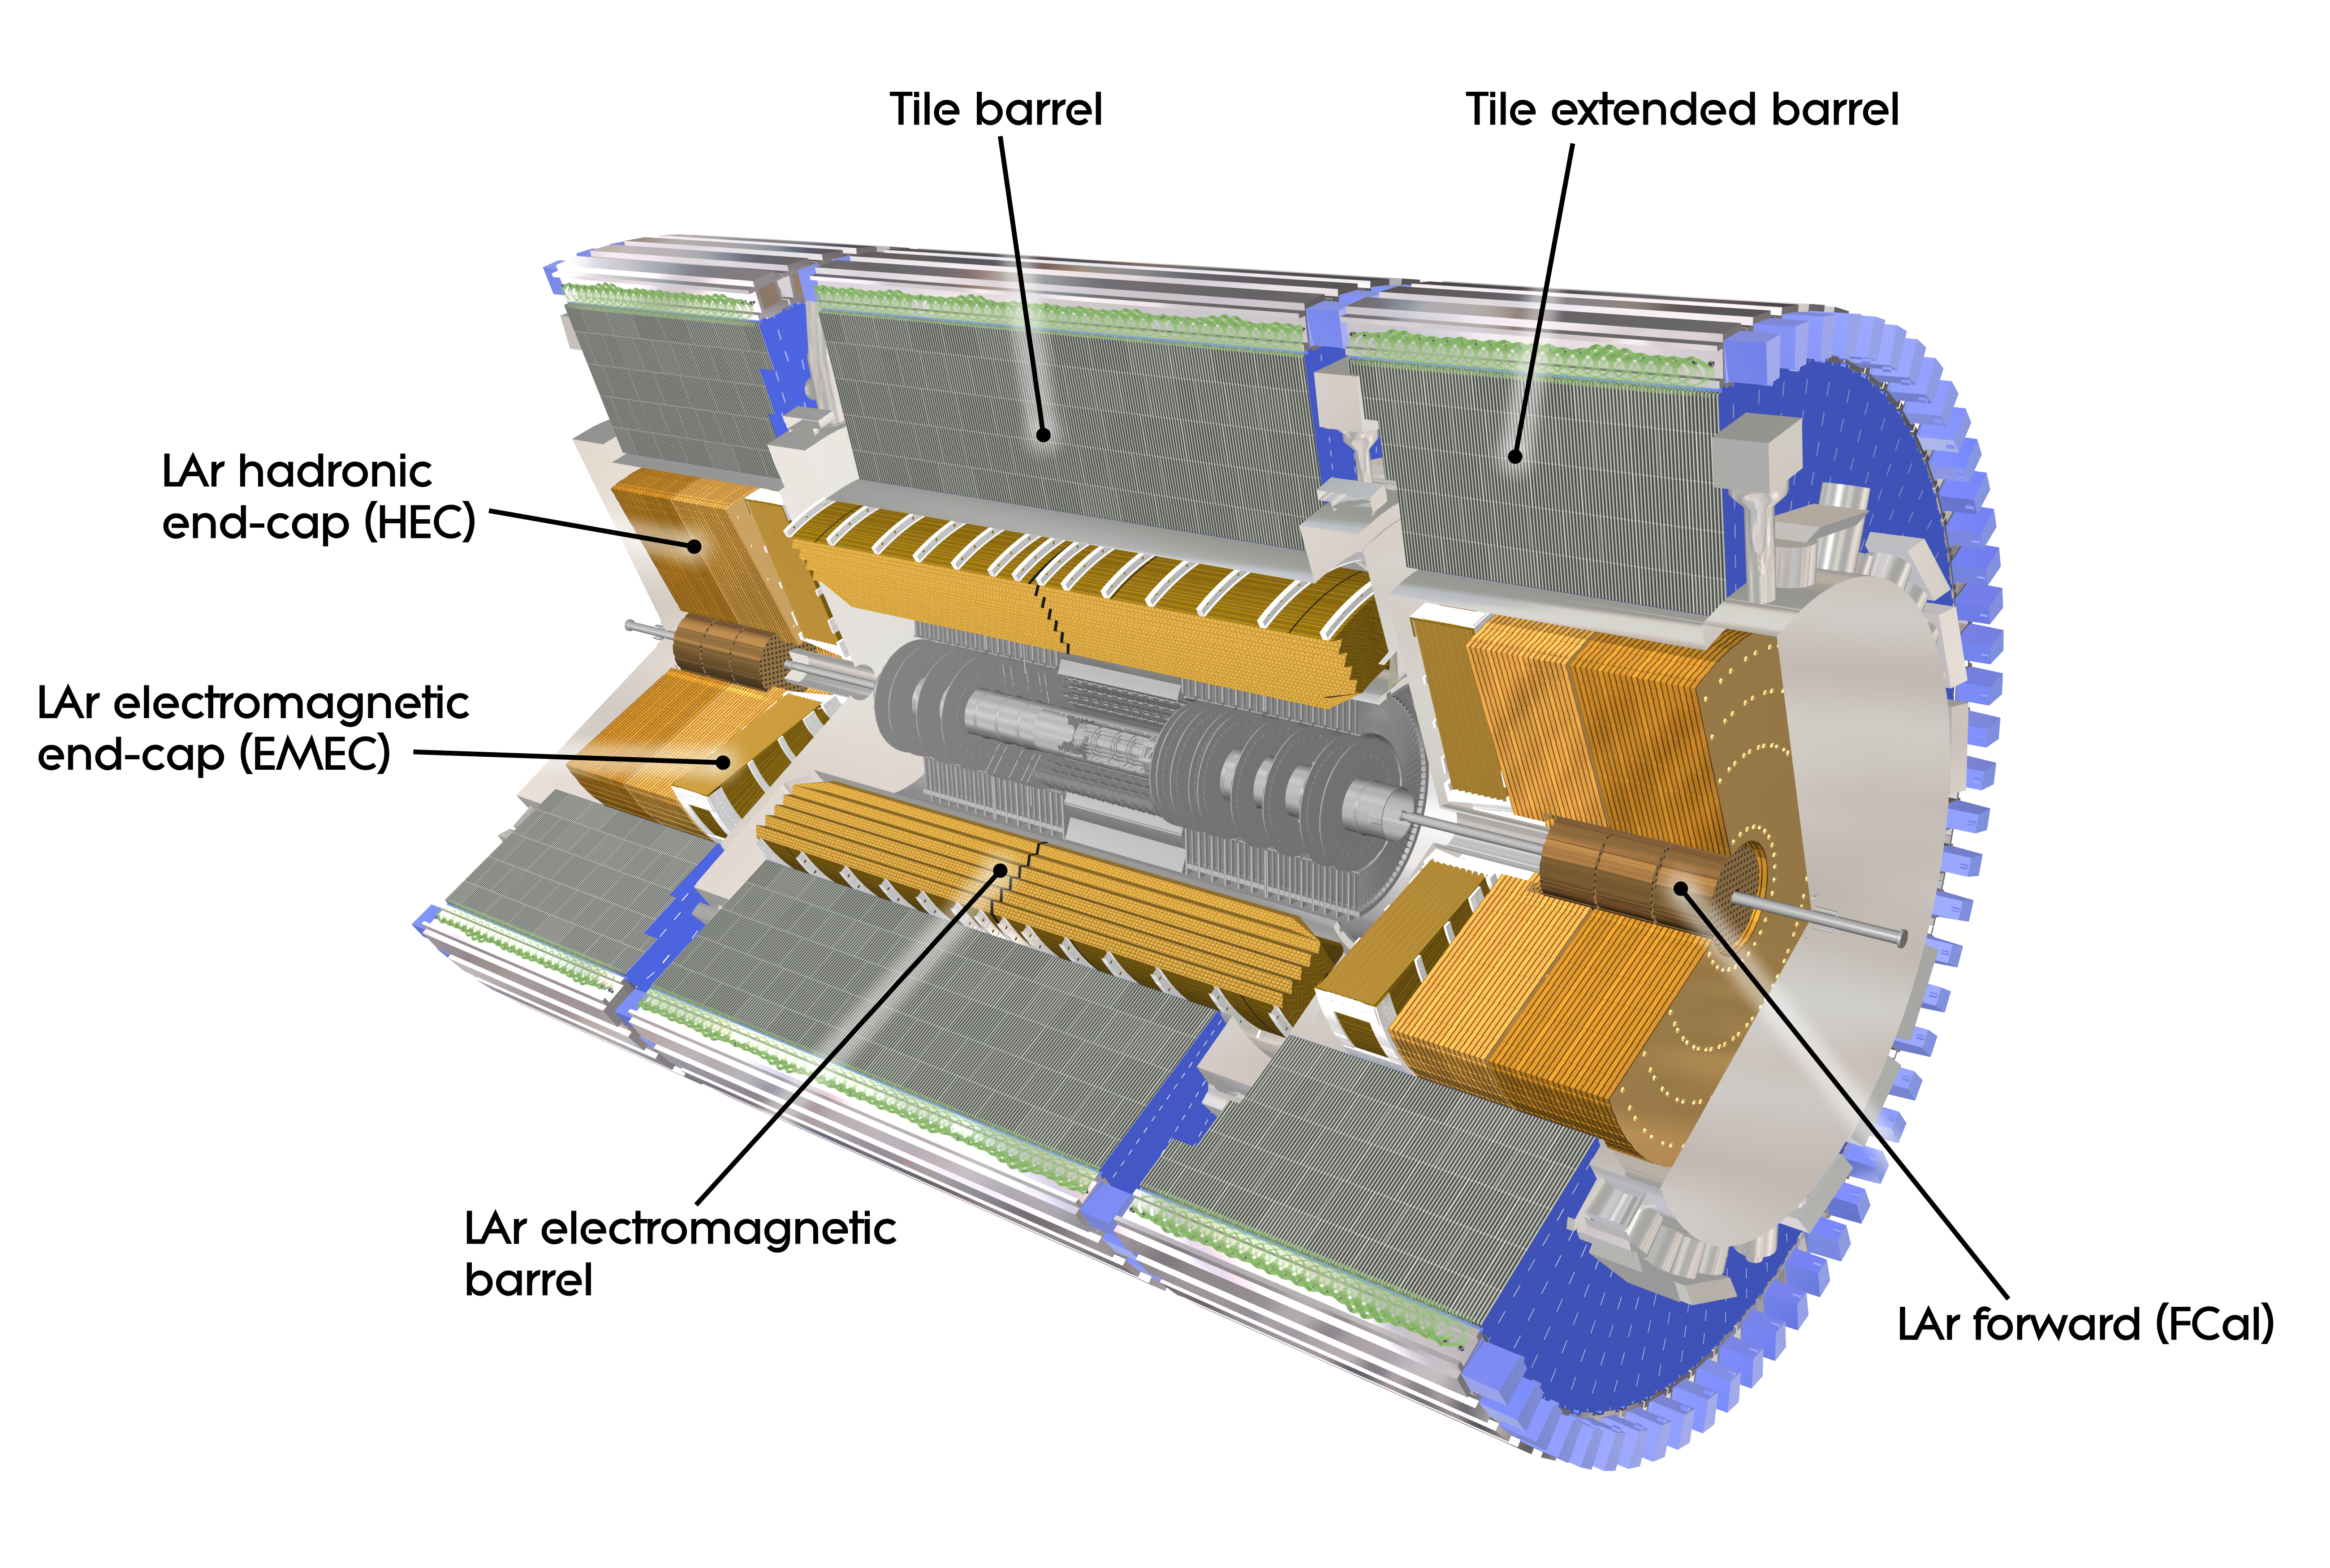
\includegraphics[width=0.8\linewidth]{3_experiment/atlas/calorimenters.jpg}
    \caption{Sistema de calorímetros de \ac{ATLAS}, mostrando el \acf{ECAL} y el \acf{HCAL}~\cite{ATLAS-Calorimeter-Diagram}.}
    \label{fig:atlas:atlas:atlas_calorimeters}
\end{figure}

El sistema \ac{ID} está rodeado por dos calorímetros: el \acf{ECAL} y el \acf{HCAL}, como se muestra en la \Fig{\ref{fig:atlas:atlas:atlas_calorimeters}}. Estos calorímetros están diseñados para medir la energía y la posición de las partículas incidentes, a través de la energía depositada por las cascadas de partículas secundarias producidas por las incidentes. Cubre todo el rango \(\phi\) y hasta el \(\abseta<4.9\), con una granularidad más fina en la región que coincide con el \ac{ID}.
El sistema de calorímetro permite discriminar entre fotones y electrones de hadrones (jets). Además, permite medir el desequilibrio energético (gracias a su cobertura total y hermiticidad) y proporciona al sistema de trigger la información necesaria para la selección de eventos.

Ambos calorímetros son denominados calorímetros de muestreo, con capas alternas de material absorbente y activo. La capa absorbente desencadena una lluvia de partículas consecutivas con el material detector, la capa activa detecta la señal.
El desarrollo de la lluvia y sus propiedades son de vital importancia para la identificación de las partículas, como se verá más adelante.
Dos magnitudes importantes en relación con los calorímetros son la longitud de radiación, $X_0$, y la longitud de interacción $\lambda$. La longitud de radiación se refiere a la distancia después de la cual la energía de una partícula (electrones por ejemplo) se ha reducido a \(1/e\) de su energía inicial. La longitud de interacción describe el camino libre medio antes de que se produzca una interacción hadrónica.

La resolución de diseño del sistema sobre la energía calorimétrica viene dada por
\begin{equation}
    \frac{\sigma(E)}{E} = 
    \frac{a}{\sqrt{E}} \oplus b \oplus \frac{c}{E}
\end{equation}
donde \(\oplus\) significa que los términos se suman en cuadratura. El término estocástico \(\frac{a}{\sqrt{E}}\) está relacionado con las fluctuaciones en los desarrollos de la lluvia, el término constante \(b\) tiene en cuenta las inhomogeneidades del detector, y el último término está asociado con el ruido electrónico y es proporcional a \(\frac{1}{E}\). El valor de los coeficientes \(a\) y \(b\) depende de los objetos incidentes. Para el caso de los electrones en el \ac{ECAL}, \(a\sim 10\%~\gev^{1/2}\) y \(b~\sim 0.7\%\), mientras que los de los piones cargados en el centro del detector son \(a~\sim50\%~\gev^{1/2}\) y \(b\sim5\%\) \cite{ATLAS-Calorimeters-PerformanceRun2}.



\subsubsection{\acf{ECAL}}
\label{subsubsec:atlas:atlas:cals:ecal}

El \ac{ECAL} está especializado en la detección de electrones, positrones y fotones, que depositan su energía en lluvias relativamente densas: electrones energéticos que irradian fotones Bremsstrahlung, mientras que los fotones energéticos se convierten en pares electrón-positrón al atravesar el material denso.
El material absorbente está hecho de plomo (Pb) con láminas de acero inoxidable, mientras que el \ac{LAr} se utiliza como material activo con electrodos de cobre y kaptón para la lectura.


El calorímetro tiene una geometría de acordeón que proporciona una simetría completa \(\phi\) sin fisuras azimutales.
Está dividido en dos medios barriles que cubren la región central del detector (\(\abseta<1.475\)), con un pequeño hueco (4 mm) en $z = 0$ y una tapa final a cada lado del haz (\(1.375<\abseta<3.2\)).
La región de transición entre el barrel y end-cap se denomina región \textit{crack}, y la mayoría de los análisis físicos que utilizan el \ac{ECAL} requieren que los fotones y electrones se encuentren fuera de ella.
Además el \ac{LAr} se utiliza para las tapas de los calorímetros hadrónicos, así como en el \acf{FCAL} ($3.1 < \eta < 4.9$).

El grosor de \ac{ECAL} es superior a 22 longitudes de radiación (\(X_0\)) en la región del barrel, mientras que es superior a \(24 X_0\) en la región de end-caps. En el caso de los fotones, la distancia a la que la energía baja a \(1/e\) es de \(9/7 X_0\), por lo que toda la energía electromagnética del fotón se deposita en el \ac{ECAL}, y sólo una pequeña parte llega al \ac{HCAL}.

El modo de medición es el siguiente. Las partículas incidentes interactúan con el medio absorbente (Pb), iniciando una lluvia de partículas cargadas y neutras. Las partículas cargadas ionizan el \ac{LAr} y los electrodos recogen los electrones producidos en el proceso de ionización. La señal total del medio activo es entonces proporcional a la energía real total de la partícula incidente.

\begin{figure}[ht!]
    \centering
    \includegraphics[width=0.8\linewidth]{3_experiment/atlas/ecal_cells}
    \caption{Segmento del \ac{ECAL} mostrando la disposición de las capas y celdas del calorímetro. Además, se muestran las dimensiones de las celdas en cada capa~\cite{ATLAS}.}
    \label{fig:atlas:atlas:cals:ecal:ecal_cells}
\end{figure}

\begin{figure}[ht!]
    \centering
    \includegraphics[width=0.46\linewidth]{3_experiment/atlas/ecal_radiation_lengths1}
    \includegraphics[width=0.46\linewidth]{3_experiment/atlas/ecal_radiation_lengths2}
    \caption{Longitudes de radiación en función de \abseta para cada capa del \ac{ECAL}~\cite{ATLAS}.}
    \label{fig:atlas:atlas:cals:ecal:ecal_radiation_length}
\end{figure}

Dentro de la región aceptada para las medidas de precisión (\(\abseta<2.5\) excluyendo el crack), el \ac{ECAL} se segmenta en tres capas longitudinales, mostradas en la \Fig{\ref{fig:atlas:atlas:cals:ecal:ecal_cells}}.
La primera capa consiste en bandas de granularidad fina (también llamada \textit{strip layer}) que ayuda a discriminar entre fotones aislados y pares de fotones espacialmente cercanos procedentes de decaimientos \(\pizero\to\gamma\gamma\). Esta capa tiene un espesor constante de \(\sim 6 X_0\) en función de \(\eta\) (véase la \Fig{\ref{fig:atlas:atlas:cals:ecal:ecal_radiation_length}}), y proporciona una medida precisa de \(\eta\).
Para los fotones y electrones de alta energía, la mayor parte de su energía se recoge en la segunda capa, que tiene una granularidad lateral de \(0.025 \times 0.025\) en \((\eta, \phi)\) y un espesor de \(\sim 24 X_0\).
La tercera capa recoge la energía depositada por las colas de la lluvia electromagnética, con un espesor que varía entre 2 y 12 \(X_0\).
También hay un \textit{presampler} (no se muestra en las figuras), que cubre la región \(\abseta<1.8\) que mejora la medición de la energía para las partículas que comienzan la lluvia antes de entrar en el calorímetro.




\subsubsection{\acf{HCAL}}



Tres capas de calorímetro hadrónico rodean el \ac{ECAL} y proporcionan discriminación adicional para electrones y fotones al medir la energía hadrónica. El \ac{HCAL} se extiende en pseudorapidez hasta \(\abseta<4.9\), permitiendo cubrir prácticamente la totalidad del ángulo sólido desde el punto de interacción. En la región del barrel (\(\abseta<1.7\)) se encuentra el primer calorímetro, el \textit{Tile calorimeter}, un calorímetro de muestreo que utiliza acero como material absorbente y tejas centelladoras como material activo~\cite{ATLAS-Tile-TDR}. Está dividido en dos partes: \(\abseta<1.0\) y \(0.8<\abseta<1.7\). Las tejas centelleadoras están dispuestas de una forma periódica y están conectadas a una fibra óptica que transporta la luz producida por las partículas que pasan a un tubo fotomultiplicador. Este arreglo se extiende, en \(R\), de 2.28 a 4.25 m. En la región del end-cap (\(1.5<\abseta<3.2\)) hay un calorímetro de muestreo hadrónico, el \acf{HEC}, con placas de cobre como absorbente y argón líquido como material activo. Cada lado del endcap consiste en dos ruedas, una detrás de la otra con las placas planas de Cu dispuestas perpendicularmente al eje del haz, con un radio de 2.3 m. Finalmente está el \ac{FCAL}, un calorímetro de muestreo que extiende la cobertura del sistema hasta \(\abseta<4.9\), coaxial al eje del haz y situado a 4.7 m a cada lado del punto de interacción. El material principal de los módulos es el \ac{LAr} (con cobre o tungsteno), y aunque no se utiliza para mediciones de precisión, proporciona información para el cálculo de la energía transversa faltante y la reconstrucción de jets en regiones muy cercanas al eje del haz.

El \ac{HCAL} tiene un espesor superior a \(7.7~\lambda\) en la región del barrel (\(9.7~\lambda\) en total si se cuenta el \ac{ECAL}). Análogamente a la longitud de radiación mencionada para el \ac{ECAL}, se puede definir la longitud de interacción hadrónica como la distancia media a lo largo de la cual la energía de un hadrón se reduce a \(1/e\) de su energía inicial. Así, toda la energía con la que los hadrones llegan al \ac{HCAL} se deposita allí.





\subsection{\acf{MS}}

\begin{figure}[ht!]
    \centering
    \includegraphics[width=0.6\linewidth]{3_experiment/atlas/muon_detector}
    \caption{Diagrama del \acf{MS}~\cite{ATLAS}.}
    \label{fig:atlas:atlas:muon_spectrometer:muon_spectrometer}
\end{figure}

Los muones de alto \pt generados en el punto de interacción tienen un poder de penetración muy elevado y son poco interactivos. Por lo tanto, el \ac{MS} \cite{ATLAS-Muon-TDR} está situado en la parte más externa del detector \ac{ATLAS}, insertado dentro del campo magnético de 4 T generado por los imanes toroidales del barrel y end-caps, y está diseñado para obtener medidas de posición y momento con alta precisión de los muones de alto \pt en un rango de \abseta de \(\abseta<2.7\). Se trata del mayor subdetector y el que da a \ac{ATLAS} su tamaño. Este subdetector se muestra en la \Fig{\ref{fig:atlas:atlas:muon_spectrometer:muon_spectrometer}}, destacando los subsistemas.

El \ac{MS} se compone de diferentes tipos de cámaras de detección (véase la \Fig{\ref{fig:atlas:atlas:muon_spectrometer:muon_spectrometer}}). Los \acp{MDT} son responsables de la mayoría de las medidas de precisión y cubren el rango de pseudorapidez hasta \(\abseta<2.7\). Funcionan de forma similar al \ac{TRT}, con tubos llenos de un gas ionizante y un ánodo central que recoge los electrones producidos, y el tiempo de deriva está asociado a la distancia a la traza dejada por la partícula. En la región del endcap se encuentran las \acp{CSC} que tienen una alta resolución espaciotemporal y una cobertura de \(\abseta>2.0\). Estas cámaras funcionan midiendo la carga depositada en un ánodo como resultado de la cascada de electrones creada cerca de él. Las \acp{RPC} proporcionan una estimación rápida del momento de los muones a nivel de trigger con una cobertura de \(\abseta<1.05\)\footnote{Durante el \ac{LS2}, la capa del end-cap ma\'s interna ha sido reemplazada por las \acp{NSW}~\cite{ATLAS-NSW}. Presenta MicroMegas como rastreadores de precisión ya que proporcionan un mejor rendimiento a las altas tasas esperadas en las futuras operaciones del LHC.}. Las \acp{RPC} miden la descarga entre dos placas resistivas paralelas sometidas a una elevada diferencia de potencial, siguiendo la ionización del volumen de gas interno causada por el paso de muones energéticos. Por último, en la región del endcap, se encuentran los \acp{TGC}, de función similar a los \acp{CSC}. También proporcionan información al sistema de trigger en esta región y tienen una cobertura de \(\abseta<2.4\).

Si los hits en el \ac{ID} y el \ac{MS} se pueden asociar a un solo muón, se obtiene una muy buena resolución del momento de hasta
\begin{equation}
    \frac{\sigma(\pt)}{\pt} = 
    0.02\% \cdot \pt~[\gev] \oplus 2\%,
\end{equation}
la cual se degrada si sólo se identifica una traza en uno de los dos sistemas.






\subsection{El sistema de Trigger}



El sistema de trigger de \ac{ATLAS}~\cite{ATLAS-Trigger-Performance-2010,ATLAS-Trigger-Performance-2015,ATLAS-Trigger-Performance-Run2} utiliza información del detector para rechazar eventos que no son de interés para el programa de \ac{ATLAS} (colisiones \textit{soft}, por ejemplo), reduciendo la frecuencia de eventos de 40 MHz (frecuencia de cruce de bunches mencionada en la \Sect{\ref{sec:atlas:LHC}}) a alrededor de 1.5 kHz. Es necesario enfatizar aquí el papel central del sistema de trigger para el correcto funcionamiento de todo el experimento, siendo el responsable de decidir qué eventos se almacenan para su posterior análisis, que podría llevar, por ejemplo, a un descubrimiento. Para lograr tal reducción en la frecuencia de eventos y, al mismo tiempo, tener una alta eficiencia en la selección de los de interés, el sistema de trigger se compone de dos niveles consecutivos capaces de realizar una identificación de partículas cada vez más compleja; un primer nivel de trigger basado en hardware, el \acf{L1}, y luego un trigger de alto nivel basado en software, el \acf{HLT}. Cada nivel permite analizar los eventos con mayor detalle, aumentando la precisión de los criterios de selección y la complejidad de los algoritmos utilizados.


\subsubsection{\acf{L1}}

La decisión del trigger comienza con el \ac{L1}, basado en hardware~\cite{ATLAS-L1Trigger}, que identifica lo que se conoce como \ac{ROI}. La \ac{ROI} consiste en celdas vecinas en los \ac{ECAL} y \ac{HCAL}, y se define a partir de la posición en el calorímetro de cada objeto encontrado en un evento potencialmente interesante, que se extiende como un cono desde el punto de interacción a lo largo del detector.
En cuanto a los muones, toma la información leída por el \ac{MS}, más concretamente por el \ac{TGC} y el \ac{RPC}, y permite obtener una estimación rápida del \pt del muón.
El \ac{L1} también tiene una componente que permite tener en cuenta los requisitos topológicos, como las selecciones de masa invariante y las medidas de distancia, denominado el \ac{L1Topo}.

El diseño del \ac{L1} permite tener una aceptabilidad en el rango de \(\abseta<2.5\) para electrones, fotones, muones y taus, hasta \(\abseta<3.2\) para jets, y \(\abseta<4.9\) para el cálculo del momento transverso faltante.
Utilizando las \acp{ROI}, el trigger \ac{L1} debe tomar la decisión de guardar o descartar el evento, reduciendo la tasa de eventos de 40 MHz a menos de 100 kHz en aproximadamente \(2.5~\mu s\), tiempo determinado en parte por el tamaño limitado de los buffers de memoria y en parte por el tiempo que tardan los muones producidos en el evento en llegar al \ac{MS}. Esta decisión final la toma el \ac{CTP}, y luego pasa las \acp{ROI} al siguiente nivel de trigger: el \ac{HLT}.



\subsubsection{\acf{HLT}}


Cuando un evento es aceptado por el \ac{L1}, el \ac{HLT}~\cite{ATLAS-HLTTrigger} ejecuta una secuencia de algoritmos a partir de las \acp{ROI} definidas por el \ac{L1}, y permite reducir la tasa de eventos que se almacena a 1.5 kHz en 0.2 s.
La reconstrucción e identificación de partículas candidatas en el \ac{HLT} se evalúa en una secuencia de pasos donde se aplican diferentes algoritmos.
Si la selección falla en un determinado paso, los pasos siguientes ya no se ejecutan para ahorrar tiempo de ejecución.
En el \ac{HLT}, los algoritmos se agrupan en conjuntos de algoritmos de reconstrucción rápida que se ejecutan en primer lugar y, a continuación, se ejecuta un conjunto de algoritmos de reconstrucción de precisión similares a los utilizados \textit{offline}.
Los algoritmos de reconstrucción rápida utilizan la información del calorímetro y de las trazas del \ac{ID} sólo dentro de la \ac{ROI} para realizar la selección e identificación de candidatos, y llevar a cabo el rechazo del fondo lo más rápido posible.
Si la partícula candidata supera los criterios definidos por la selección de reconstrucción rápida, se ejecutan los algoritmos de selección de precisión. Estos tienen acceso a la información del detector fuera de la \ac{ROI}, con la máxima granularidad e incluyendo detalles sobre la calibración energética del calorímetro, la alineación del subdetector y el mapeo del campo magnético.

La secuencia exacta y el tipo de algoritmos considerados en el \ac{HLT} se definen en el \textit{menu} del trigger. Esto comprende una base de datos de triggers, cada uno de los cuales define una secuencia de algoritmos y los requisitos de estos algoritmos para que un evento pase el \ac{HLT}.

Los requisitos de trigger se diseñan de forma tal que la tasa global del \ac{HLT} no supere 1 kHz. En algunos casos, incluso la reducción de la tasa de eventos conseguida mediante los algoritmos del \ac{HLT} para los requisitos de trigger deseados, como los trigger para objetos con bajo momento, es demasiado alta. Para mantener la tasa general del \ac{HLT} por debajo de 1 kHz en estos casos, los triggers pueden seguir incluyéndose en el menú, pero con una preescala. Un preescalado es un escalado artificial del trigger, que sólo acepta la N-ésima decisión de trigger si el factor de preescalado es N. Esto permite que los triggers con una alta tasa sigan recogiendo eventos.

Los algoritmos del \ac{HLT} se ejecutan en aproximadamente 40.000 núcleos de CPU. Además, la construcción parcial de eventos se utiliza para análisis a nivel de trigger, para el monitoreo del detector y las calibraciones del subsistema detector. Finalmente, los eventos aceptados por el \ac{HLT} se almacenan y se distribuyen, disponibles \textit{offline} para cualquier estudio o análisis.






\FloatBarrier
\section{Toma de datos durante el Run-2}
\label{sec:atlas:runs}


El funcionamiento del \ac{LHC} se organiza en distintos períodos conocidos como \textit{runs}.
% Cada run suele durar varios años y se caracteriza por condiciones experimentales específicas, como la energía a la que colisionan los protones y la intensidad de los haces.
Desde su puesta en marcha, se pueden distinguir los siguientes runs: Run-1 (2010-2013) operó a energías de colisión de hasta 8 TeV, Run-2 (2015-2018) a 13 TeV, y Run-3 (2022-presente) a 13.6 TeV. Cada período de toma de datos, una vez que el \ac{LHC} anuncia haces estables, se divide en \ac{LB} de aproximadamente dos minutos. En cada \ac{LB}, la luminosidad instantánea es prácticamente constante y las condiciones del haz son estables. Debido a la alta complejidad del \ac{LHC} y del detector \ac{ATLAS}, se espera que haya ineficiencias en los detectores y subdetectores y/o en la cadena de adquisición de datos. Durante cada run, cada parte del \ac{ATLAS} es monitoreada y cualquier falla o problema es registrado, incluyendo componentes inactivos, o problemas en el haz del \ac{LHC}.

Para garantizar la alta calidad de los datos, libres de defectos significativos, los \ac{LB} y los rangos dentro de ellos que superan todos los criterios de calidad se compilan en \ac{GRL}. Las listas se elaboran y distribuyen de forma centralizada, con el fin de proporcionar a cualquier grupo de \ac{ATLAS} la misma colección de \acp{LB}. Dado que durante los períodos de tomas de datos están disponibles diferentes partes del detector (en un run óptimo, todos los subdetectores están disponibles), hay múltiples \acp{GRL} disponibles para utilizar. Cada análisis, entonces, selecciona qué \ac{GRL} utilizar dependiendo de su tolerancia a las fallas de los subdetectores.

La presente tesis utiliza datos recolectados por \ac{ATLAS} de colisiones \pp del \ac{LHC} durante el Run-2 (2015-2018), a una energía del centro de masa de \(\sqrt{s} = 13~\tev\). Durante este run, el \ac{LHC} entregó un total de \(156~\ifb\), de los cuales \ac{ATLAS} recolectó \(147~\ifb\). La luminosidad integrada total disponible para análisis de física es de \(140.07~\ifb\)\footnote{Las primeras medidas y \ac{GRL} iniciales sólo brindaban un total de \(139~\ifb\) disponibles para análisis}, como se ve en la \Fig{\ref{fig:atlas:runs:lumi_run2}}. La incertidumbre en la luminosidad integrada combinada para el Run-2 es de \(0.83\%\)~\cite{ATLAS-Lumi-Run2}, obtenida usando el detector LUCID-2~\cite{ATLAS-LUCID2}.
Hasta el momento, combinando los años 2022, 2023 y 2024 de toma de datos del Run-3, se recogieron 159 \ifb de datos, mostrados en la \Fig{\ref{fig:atlas:runs:lumi_run3}}~\cite{ATLAS-Lumi-Run3-2022,ATLAS-Lumi-Run3-2023}.

\begin{figure}[ht!]
    \centering
    \begin{subfigure}[h]{0.46\linewidth}
        \centering
        \includegraphics[width=\linewidth]{3_experiment/lhc/DeliveredLuminosityRun2}
        \caption{Run-2 (2015-2018)}
        \label{fig:atlas:runs:lumi_run2}
    \end{subfigure}
    \hfill
    \begin{subfigure}[h]{0.46\linewidth}
        \centering
        \includegraphics[width=\linewidth]{3_experiment/lhc/DeliveredLuminosityRun3}
        \caption{Early Run-3 (2022-2024)}
        \label{fig:atlas:runs:lumi_run3}
    \end{subfigure}
    \caption{Luminosidad entregada por el \ac{LHC} y recolectada por \ac{ATLAS} durante el Run-2~\cite{ATLAS-Lumi-Run2} y el Run-3. En el caso de Run-2, también se muestra la fracción de datos recolectados que son útiles para análisis de física.}
    \label{fig:atlas:runs:lumi}
\end{figure}

Otro concepto importante en la adquisición de datos en \ac{ATLAS} es el \textit{pileup}, que se produce cuando las partículas producidas en más de una colisión \pp llegan al detector al mismo tiempo, o más generalmente, cuando las señales se solapan de forma que no pueden separarse. Cuando colisionan haces de protones, la probabilidad de que se produzca una interacción es proporcional a la densidad de partículas, o mejor, al flujo de partículas, que se expresa mediante la luminosidad instantánea. El número real de colisiones de partículas que tienen lugar cuando dos haces se cruzan es una variable aleatoria que sigue una distribución de Poisson. Para luminosidades bajas, en la mayoría de los cruces de haces no se produce ninguna colisión, pero para luminosidades instantáneas altas, en la mayoría de los cruces se producen muchas colisiones simultáneas entre partículas. Dependiendo del subdetector y del tipo de medida, puede o no ser posible distinguir entre partículas procedentes de diferentes interacciones simultáneas. Es lo que se denomina como \textit{in-time pileup}. Por el contrario, el \textit{out-of-time pileup} incluye los efectos que surgen cuando el tiempo que el detector necesita para volver a su estado de espera es mayor que el tiempo entre cruces de haces. Una medida cuantitativa del pileup y de la actividad de eventos es el valor medio de interacciones inelásticas \pp por bunch-crossing, \avgmu.

Las luminosidades instantáneas máximas se multiplicaron por cuatro a lo largo de los cuatro años del Run-2, resultando en un aumento de \avgmu desde 10 hasta 60, como se muestra en la \Fig{\ref{fig:atlas:runs:pileup_run2}}. Para el Run-3, el pileup aumentó drásticamente hasta valores de 57 para el año 2024, aumentando en promedio hasta 52 interacciones por bunch-crossing, mostradas en la \Fig{\ref{fig:atlas:runs:pileup_run3}}.

\begin{figure}[ht!]
    \centering
    \begin{subfigure}[h]{0.46\linewidth}
        \centering
        \includegraphics[width=\linewidth]{3_experiment/lhc/PileupConditionsRun2.png}
        \caption{Run-2}
        \label{fig:atlas:runs:pileup_run2}
    \end{subfigure}
    \hfill
    \begin{subfigure}[h]{0.46\linewidth}
        \centering
        \includegraphics[width=\linewidth]{3_experiment/lhc/PileupConditionsRun3.png}
        \caption{Run-3}
        \label{fig:atlas:runs:pileup_run3}
    \end{subfigure}
    \caption{Distribución del número de interacciones por bunch-crossing durante Run-2 (izquierda) y Run-3 (derecha).}
    \label{fig:atlas:runs:pileup}
\end{figure}